%%%%%%%%%%%%%%%%%%%%%%%%%%%%%%%%%%%%%%%%%
% Short Sectioned Assignment LaTeX Template Version 1.0 (5/5/12)
% This template has been downloaded from: http://www.LaTeXTemplates.com
% Original author:  Frits Wenneker (http://www.howtotex.com)
% License: CC BY-NC-SA 3.0 (http://creativecommons.org/licenses/by-nc-sa/3.0/)
%%%%%%%%%%%%%%%%%%%%%%%%%%%%%%%%%%%%%%%%%

%----------------------------------------------------------------------------------------
%	PACKAGES AND OTHER DOCUMENT CONFIGURATIONS
%----------------------------------------------------------------------------------------

\documentclass[paper=a4, fontsize=10pt]{article} % A4 paper and 11pt font size


\usepackage[vmargin=2.5cm,hmargin=3cm]{geometry}
% ---- Entrada y salida de texto -----

\usepackage[T1]{fontenc} % Use 8-bit encoding that has 256 glyphs
\usepackage[utf8]{inputenc}
\usepackage{helvet}
\renewcommand{\familydefault}{\sfdefault}
%\usepackage{fourier} % Use the Adobe Utopia font for the document - comment this line to return to the LaTeX default

% ---- Idioma --------

\usepackage[spanish, es-tabla]{babel} % Selecciona el español para palabras introducidas automáticamente, p.ej. "septiembre" en la fecha y especifica que se use la palabra Tabla en vez de Cuadro

% ---- Otros paquetes ----
\usepackage[hidelinks]{hyperref} % Estilo para los enlaces
\hypersetup{
  colorlinks   = true, %Colours links instead of ugly boxes
  urlcolor     = blue, %Colour for external hyperlinks
  linkcolor    = black, %Colour of internal links
  citecolor   = blue %Colour of citations
}
\usepackage{url} % ,href} %para incluir URLs e hipervínculos dentro del texto (aunque hay que instalar href)
\usepackage{amsmath,amsfonts,amsthm} % Math packages
%\usepackage{graphics,graphicx, floatrow} %para incluir imágenes y notas en las imágenes
\usepackage{graphics,graphicx, float} %para incluir imágenes y colocarlas

%Para incluir codigo
\usepackage{minted}

% Para hacer tablas comlejas
%\usepackage{multirow}
%\usepackage{threeparttable}

%\usepackage{sectsty} % Allows customizing section commands
%\allsectionsfont{\centering \normalfont\scshape} % Make all sections centered, the default font and small caps

\usepackage{fancyhdr} % Custom headers and footers
\pagestyle{fancyplain} % Makes all pages in the document conform to the custom headers and footers
\fancyhead{} % No page header - if you want one, create it in the same way as the footers below
\fancyfoot[L]{} % Empty left footer
\fancyfoot[C]{} % Empty center footer
\fancyfoot[R]{\thepage} % Page numbering for right footer
\renewcommand{\headrulewidth}{0pt} % Remove header underlines
\renewcommand{\footrulewidth}{0pt} % Remove footer underlines
\setlength{\headheight}{13.6pt} % Customize the height of the header

\numberwithin{equation}{section} % Number equations within sections (i.e. 1.1, 1.2, 2.1, 2.2 instead of 1, 2, 3, 4)
\numberwithin{figure}{section} % Number figures within sections (i.e. 1.1, 1.2, 2.1, 2.2 instead of 1, 2, 3, 4)
\numberwithin{table}{section} % Number tables within sections (i.e. 1.1, 1.2, 2.1, 2.2 instead of 1, 2, 3, 4)

\setlength\parindent{0pt} % Removes all indentation from paragraphs - comment this line for an assignment with lots of text

\newcommand{\horrule}[1]{\rule{\linewidth}{#1}} % Create horizontal rule command with 1 argument of height


%------------------------------------------------------------------------
%	TÍTULO Y DATOS DEL ALUMNO
%------------------------------------------------------------------------

\title{	
\normalfont \normalsize 
\textsc{\textbf{Ingeniería de Servidores (2016-2017)} \\ Grado en Ingeniería Informática \\ Universidad de Granada} \\ [25pt] % Your university, school and/or department name(s)
\horrule{0.5pt} \\[0.4cm] % Thin top horizontal rule
\huge Comparativa entre systemd e init. \\ % The assignment title
\horrule{2pt} \\[0.5cm] % Thick bottom horizontal rule
}

\date{\normalsize\today} % Incluye la fecha actual

%-------------------------------------------------------------------------
% DOCUMENTO
%-------------------------------------------------------------------------

\begin{document}

\maketitle % Muestra el Título

\newpage

%-------------------------------------------------------------------------
%	Resumen introductorio (entre 5 y 15 lineas)
%----------------------------------------------------------------------
\begin{abstract}

En el mundo de \textit{UNIX} donde el kernel está público y cada vez es más grande la comunidad que lo desarrolla, aparecen nuevas contribuciones para intentar mejorar el sistema. En nuestro caso vamos a analizar una nueva implementación del ``proceso 1'' que rápidamente ha sido adaptada por las principales distribuciones de \textit{UNIX}, \texttt{systemd}, sustituyendo al proceso \texttt{init}. Explicaremos en que consiste tanto \texttt{systemd} como \texttt{init} con sus ventajas e inconvenientes, además analizaremos en profundidad \texttt{systemd}, ya que es la nueva tecnología que utilizan prácticamente todas las distribuciones de \texttt{Linux} actuales. Por último haremos una conclusión final dando una valoración sobre estos procesos aplicados en el mundo de los servidores.



\end{abstract}

%--------------------------------------------------------------------------
%	Introducción
%-------------------------------------------------------------------------

\section{Introducción} % máximo 2 páginas
Como se indica en la historia de The Open Group \cite{unix}, los sistemas de tipo \textit{UNIX}, concedidos a principios de la década de los 70, se idearon de forma gratuita y libre, fomentando la idea de software libre y de código abierto. Creando así la comunidad tan grande y amplia que conocemos hoy en día. Gracias a esta comunidad se ha seguido desarrollando y avanzando el sistema \textit{UNIX} hasta el kernel de \textit{Linux} que conocemos y utilizamos a diario. Constantemente se están desarrollando nuevas tecnologías y procesos para mejorar este sistema.\\

Nosotros nos vamos a centrar en comparar una nueva forma de uno de los procesos principales del sistema con su predecesor que curiosamente se ha mantenido casi intacto desde la década de los noventa, es decir, desde hace más de 20 años no ha sido modificado, hecho sorprendente pensando en la velocidad a la que avanza siempre la tecnología. El proceso en cuestión es el encargado del inicio del sistema, es el proceso con PID 1 (Proccess ID). El arranque del sistema funciona con un proceso que va ejecutando todos los demás procesos, como los drivers del adaptador de red o del ratón, los controladores de pantalla, etc.\\

Este proceso era \texttt{init} que era utilizado por todas las distribuciones basadas en Linux. Pero Lennart Poettering, como redacta en su articulo \cite{Lennart}, y Kay Sievers decidieron desarrollar un nuevo proceso de arranque del sistema, desarrollando así \texttt{systemd}, el encargado de iniciar prácticamente todas las distribuciones de Linux actuales.\\

Aunque ambos sistemas son daemons (demonios) hay multitud de diferencias entre ellos, que se explicarán mas adelante y finalmente se hará una conclusión de ambos sistemas de arranque para el mundo de los servidores.



%--------------------------------------------------------------------------
%	Init
%--------------------------------------------------------------------------

\section{Proceso init} % máximo 4 páginas
El proceso \texttt{init} se caracteriza por su simpleza y facilidad de uso. El funcionamiento de \texttt{init} consiste en ir iniciando los procesos listados en un archivo de configuración, es decir, inicia el primer proceso del listado y cuando éste se ha iniciado inicia el siguiente y así sucesivamente. De esta forma tan simple es como \texttt{init} inicia el sistema. Además utiliza la filosofía del software libre de ser transparente para el usuario y permitirle poder modificar por completo su implementación, ya que basta con modificar el fichero de configuración. De esta forma el proceso \texttt{init} siempre es el padre o antecesor de todo proceso existente en el sistema y además adopta cualquier proceso que pudiera quedarse sin un padre por el motivo que fuera.\\

Sin embargo presenta unos claros inconvenientes derivados de su propia naturaleza simple y sencilla. El primer inconveniente es el control de las dependencias, ya que deben controlarse por parte del programador y tiene que tener conocimientos de las dependencias que tienen los procesos y listar primero los procesos que no tienen dependencias o cuyas dependencias ya se han resuelto, por ejemplo si en el listado de procesos aparece un proceso apache que depende de la configuración de red este proceso se iniciará con errores o no se iniciará puesto que el controlador de red todavía no se ha iniciado, aún cuando tanto apache como el controlador de red estén perfectamente configurados. El otro inconveniente principal, sobre todo en servidores, es la sobrecarga al inicio del sistema, ya que se inician los procesos de uno en uno y hasta que uno no acabe de arrancar no se inicia el siguiente.

\subsection{System V }
Tal como se dice en el artículo de Jonas Gorauskas en ``Linux Jornal'' \cite{SysV}, \texttt{System V} fue una versión mejorada del \texttt{init} original y es la que ha estado presente todo este tiempo en las distintas distribuciones de \texttt{Linux}. Aunque esta versión de \texttt{init} sigue utilizando su estructura monolítica y por tanto mantiene el inconveniente del control de dependencia, añadía un sistema de llamadas por niveles de prioridad para la ejecución de los procesos del sistema. Este proceso de llamadas se realiza mediante un esquema de directorios con niveles de ejecución  que contienen los scripts de arranque de los servicios. Dependiendo de la distribución de \texttt{Linux} se utilizan más o menos niveles de prioridad de ejecución.\\


Como se puede observar en la figura \ref{fig:System_V} el proceso de arranque del sistema empieza en las BIOS, continuando por la llamada al GRUB que seleccionando un sistema operativo carga el Kernel. En el caso de sistemas Linux con \texttt{System V init} primero leería el fichero de configuración inittab, en el cual se indica el esquema que debe seguir los niveles de ejecución del proceso. En este caso hemos utilizado de ejemplo un sistema con 5 niveles.

\begin{figure}[H] %con el [H] le obligamos a situar aquí la figura
\centering
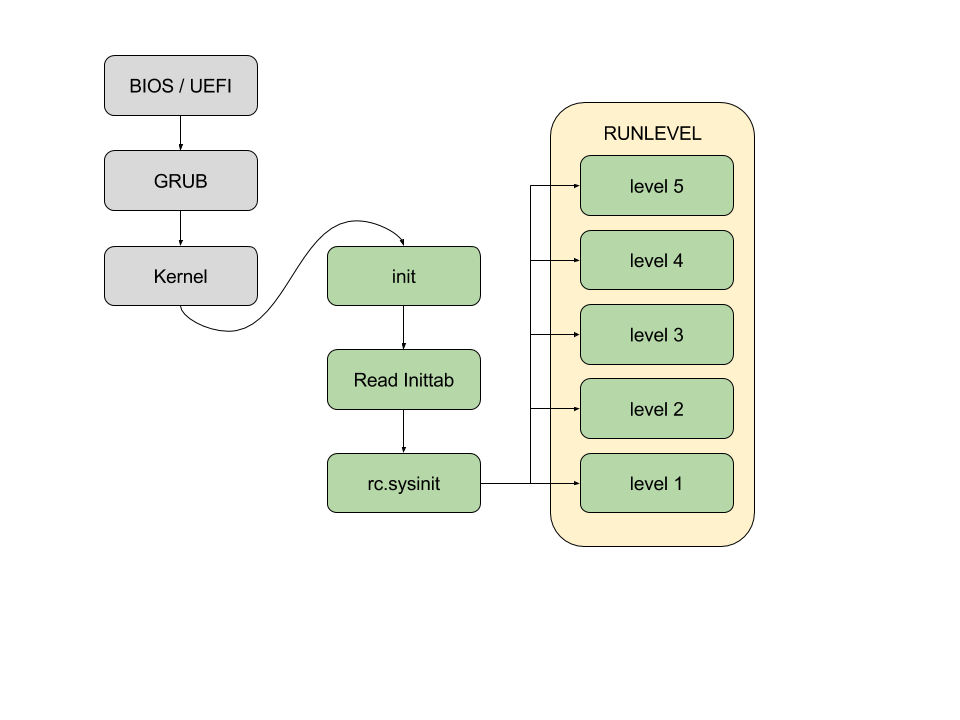
\includegraphics[scale=0.38]{./imagenes/System_V.png} 
\caption{System V - boot process} \label{fig:System_V}
\end{figure}



\subsubsection{Problemas de System V}
System V presenta una serie de problemas debido a como fue concebido, ya que se pensó para equipos estáticos y que mantenían su hardware, por ello se desarrollo de forma estática y síncrona para el arranque y apagado del sistema, dando lugar a bloqueos de tareas futuras hasta que las actuales no fueran completadas. Esto deja al sistema sin poder reaccionar ante algunos eventos que no estaban programados para el inicio o apagado del sistema. Además no había un control sobre los demonios una vez ejecutados, si estos tenían cualquier problema durante su ejecución no eran tratados por nadie, como mucho si se quedaban huérfanos los recogía el proceso \texttt{init}, pero si se paraban no volvía a lanzarlos aunque fueran procesos importantes o vitales para el sistema.
%------------------------------------------------------------------------
%	Systemd
%-------------------------------------------------------------------------

\section{Proceso systemd} % máximo 4 páginas

Como ya hemos dicho anteriormente \texttt{systemd} fue desarrollado por Lennart Poettering y Kay Sievers, ambos empleados de Red Hat.
El proceso \texttt{systemd} tal como lo definen los autores en la web oficial de \texttt{systemd} \cite{systemd} es una suite o conjunto de herramientas diseñadas para ofrecer una funcionalidad específica, en este caso para facilitar y mejorar el arranque del sistema operativo \textit{Linux}. Específicamente es un conjunto de demonios de \textit{Linux}, un demonio \cite{daemons} es un proceso que funciona en segundo plano en el sistema a la espera de eventos o llamadas que se producen en el sistema y cuando son despertados realizan una tarea concreta. Systemd no solo ha sustituido al proceso init, sino a toda la gestión que era necesaria para el correcto funcionamiento del inicio del sistema.\\

Lennart y Kay diseñaron \texttt{systemd} buscando una mayor eficiencia en el inicio de los sistemas \texttt{Linux}, para ello crearon un \texttt{framework}, un \texttt{framework} en software es una infraestructura estandarizada en resolver un problema específico donde poder expresar todas las dependencias y así poder realizar una mejor gestión de las dependencias. Para conseguir una mayor eficiencia se centraron en el paralelismo frente la ejecución de procesos de forma secuencial que utilizaba su predecesor. Ahora \texttt{systemd} realiza todas las llamadas para el inicio del sistema por lo que se ha eliminado la utilización de una terminal como intermediario, ahorrando tiempo en el inicio del sistema. El \texttt{framework} de dependencias es mucho más permisivo ya que es capaz de controlarlas a un nivel más bajo consiguiendo de esta forma ser mucho más agresivo en la paralelización del inicio del sistema. Además permite al administrador del sistema un mayor control sobre el orden en que se inician los servicios.\\


En el artículo de ZDNet \cite{zdnet} podemos ver un esquema de los componentes de systemd como se muestra en la figura \ref{fig:systemd_components}. Se pueden observar los cinco grande módulos en los que se divide la suite \texttt{systemd}: Libraries, Core, Targets, Daemons y Utilities.

\begin{figure}[H] %con el [H] le obligamos a situar aquí la figura
\centering
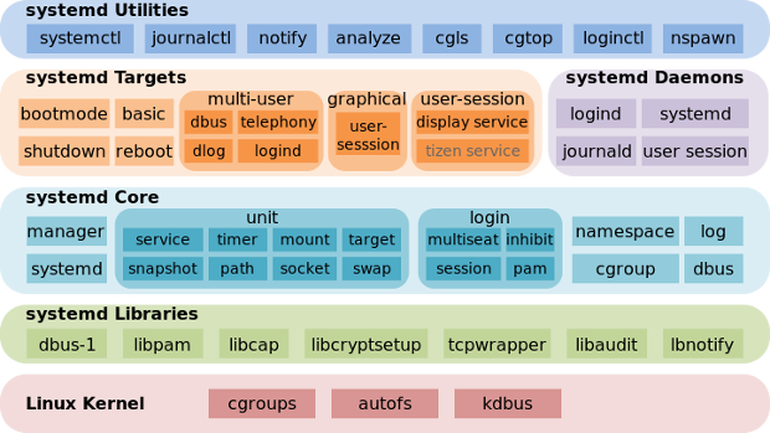
\includegraphics[scale=0.5]{./imagenes/systemd_components.png} 
\caption{Componentes de systemd} \label{fig:systemd_components}
\end{figure}

Para la resolución de dependencias se fijaron en su problema más fundamental, la utilización de servicios y comunicaciones con otros procesos. Para las comunicaciones se sirven normalmente de los \texttt{sockets}, un \texttt{socket} no es más que una estructura de datos del sistema de archivos para el intercambio de información entre procesos de un sistema \texttt{Linux}, como indica el manual (\texttt{man}) de \texttt{Linux} \cite{socket}. De esta forma se pueden iniciar todos los demás procesos de forma paralela teniendo en cuenta menos dependencias puesto que al estar los \texttt{sockets} ya creados pueden empezar la comunicación aunque alguno de los dos procesos todavía no este iniciado. Por ejemplo los procesos que necesitan escribir en los ``logs'' del sistema dependen del \texttt{socket} ``/dev/log'', entonces \texttt{systemd} crea este \texttt{socket} de los primeros, eliminando así múltiples dependencias y bloqueos a otros servicios por consecuencia de las dependencias. De esta forma se consigue que aunque el proceso no se haya iniciado, el \texttt{socket} donde tiene que leer ya esté cargado con la información necesaria y así cuando el proceso se inicie cargarla directamente. \\

Las dependencias que se mantienen después de las mejoras previamente descritas se resuelven con un sistema de ``\texttt{target}'', si en \texttt{System V} teníamos un esquema de jerarquía con niveles de ejecución en \texttt{systemd} tenemos algo parecido que sirve al mismo propósito. Como se dice en ArchLinux Wiki \cite{systemd_es}: ``\textit{Cada target se nomina, en lugar de numerarse, y está destinado a servir a un propósito específico con la posibilidad de realizar más de una acción al mismo tiempo. Algunos targets son activados heredando todos los servicios de otro target e implementando servicios adicionales. Como hay targets de systemd que imitan los runlevels de SystemV init, es, por tanto, posible pasar de un target a otro...}''.\\


La suite de \texttt{systemd} como comentamos anteriormente trae una serie de herramientas orientadas a mejorar el sistema y las opciones que puede realizar el usuario final, tal como se indican en la wiki de ArchLinux \cite{systemd_es} y en la documentación de ``SUSE'' \cite{suse_doc} incluye los demonios para el control de sesiones (\texttt{logind}), redes (\texttt{networkd}) y los mensajes del sistema (\texttt{journald}). También cuenta con utilidades como un analizador de estado del sistema, que nos muestra de forma cómoda las unidades que han tenido algún tipo de problema o simplemente las unidades instaladas en el sistema. Otra utilidad es la gestión de energía instalada en el paquete de \texttt{logind} que, por ejemplo, permite un apagado o reinicio del sistema.\\


Vamos a comentar los principales demonios de systemd:

\subsection{Demonio journald}
Para conocer un poco más en profundidad sobre este demonio vamos a consultar un articulo en el blog de Lennart \cite{Journald} en el cual se explica lo siguiente. \texttt{Journald} es un demonio incluido en la suite de \texttt{systemd} para la gestión de los mensajes del sistema que cuenta con un nuevo esquema provisto de una estructura de índices. Con esta nueva versión de demonio para los logs se mantiene la compatibilidad con los demonios anteriores y además es más eficiente que su antecesor ya que utiliza la salida estándar junto con las llamadas al sistema de forma nativa en el propio demonio.

\subsection{Demonio logind}
Este demonio, tal y como se dice en la documentación oficial de systemd \cite{man_systemd_logind}, es el encargado de administrar los inicios de sesión de los usuarios del sistema. Por lo tanto realiza un control de los usuarios y sus sesiones así como de sus procesos. La configuración de este servicio se guarda en \texttt{logind.conf}.

\subsection{Demonio user session}
Este demonio es el más sencillo, su función es permitir o bloquear los inicios de sesión de usuario dependiendo del estado del sistema \cite{man_systemd_user-sessions}.


\subsection{Implementación}

Podemos encontrar la implementación completa de systemd en su GitHub \cite{implementacion_systemd}. Por ejemplo en el archivo \texttt{src/systemd/sd-daemon.h} podemos ver la definición de los niveles de ``logs'' que utiliza el proceso \texttt{systemd}.

\begin{minted}{c}
/*
  Log levels for usage on stderr:
          fprintf(stderr, SD_NOTICE "Hello World!\n");
  This is similar to printk() usage in the kernel.
*/
#define SD_EMERG   "<0>"  /* system is unusable */
#define SD_ALERT   "<1>"  /* action must be taken immediately */
#define SD_CRIT    "<2>"  /* critical conditions */
#define SD_ERR     "<3>"  /* error conditions */
#define SD_WARNING "<4>"  /* warning conditions */
#define SD_NOTICE  "<5>"  /* normal but significant condition */
#define SD_INFO    "<6>"  /* informational */
#define SD_DEBUG   "<7>"  /* debug-level messages */
\end{minted}

Se puede observar que se definen ocho niveles de ``logs'', de más prioritario a menos, siendo 0 el más prioritario.


%-------------------------------------------------------------------------
%	Comparativa
%--------------------------------------------------------------------------

\section{Ventajas e inconvenientes de systemd frente init (system V) } 
En la web de linoxide se puede ver una comparativa \cite{systemd_vs_sysvinit} que han realizado sobre los principales comandos de Systemd frente a SysVinit. De una forma muy clara y rápida se aprecian las principales diferencias entre estos dos sistemas, como por ejemplo \texttt{systemd} utiliza el comando \texttt{systemctl <opción> <servicio>}, mientras que \texttt{Sistem V init} utiliza la estructura \texttt{service <servicio> <opción>}. Podemos ver la tabla de la comparativa completa en la figura \ref{fig:systemd_sysVinit}.




\subsection{Ventajas}
Systemd tiene mayor velocidad en el arranque del sistema, ya que utiliza la paralelización y el control de dependencias explicado anteriormente. No requiere satisfacer ciertas dependencias al momento de cargar los componentes, lo que hace que el proceso de arranque sea más rápido. Frente al arranque lento y secuencial de init.\\

Systemd realiza una supervisión de todos los procesos en PID1, teniendo la capacidad para analizar todos estos procesos.\\

Systemd tiene una mejor paralelización de servicios independientes gracias a los servicios de activación de sockets y la activación de buses, que realiza de forma tan eficiente.\\

Systemd optimiza el uso de recursos utilizando \texttt{cgrups} que administra los puntos de montaje y el montaje de unidades de almacenamiento bajo demanda.\\

Systemd es compatible con las versiones anteriores de init. De forma que systemd puede ejecutar una configuración de init sin ningún problema.

\subsection{Inconvenientes}

Systemd tiene una implementación fuertemente ligada, es decir, está ligado a un núcleo, a una librería y a un administrador de dispositivos específicos.\\

Systemd requiere de un conjunto de paquetes extra, como son: ACL, PAM, DBus y polkit. Los cuales son paquetes extra que no hacen falta realmente para iniciar el sistema. Por lo que provoca una pequeña sobrecarga del sistema.\\

Realmente no son tantos los inconvenientes encontrados frente a los avances que suponen. Aunque sí se puede encontrar un gran número de desarrolladores completamente en contra ante este nuevo sistema de arranque.

%-------------------------------------------------------------------------
%	Conclusiones
%--------------------------------------------------------------------------

\section{Conclusiones} % maximo 2 
Finalmente vamos ha hacer una pequeña conclusión referente al mundo de los servidores basándonos en todo lo explicado anteriormente.\\

En el mundo de los servidores donde es tan importante la sobrecarga del sistema producida por el propio sistema operativo y sus componentes, se va buscando siempre reducir esta sobrecarga para aumentar las prestaciones que ofrece el servidor a los clientes. Por lo tanto podría ser difícil decidir que sistema de arranque elegir, ya que systemd genera una mayor sobrecarga que init, pero lo compensa con un inicio de sistema mucho más rápido. De hecho este tema esta dividiendo a la comunidad de linux, aunque en servidores la decisión parece unánime eligiendo init frente a systemd por su menor sobrecarga del sistema, ya que en el ámbito de los servidores no es tan importante el tiempo de inicio del sistema, dado que un servidor suele estar siempre encendido y rara vez se apaga o reinicia.\\

Además se complica considerablemente las funciones del administrador del sistema, ya que al unificar tantas funciones y utilidades bajo un mismo framework no permite al administrador modularizar y distribuir según las necesidades que requiere el servidor en particular.\\

Por lo tanto podemos decir que en ordenadores de ámbito personal o domésticos se puede considerar una ventaja utilizar systemd en vez de init, ya que para el usuario estándar, el cual le da un uso normal al sistema, es preferible un inicio más rápido y una mayor abstracción de la administración del sistema teniéndolo todo unificado, como ya hacen el resto de los sistemas operativos modernos, como son Windows o Mac.\\

Sin embargo justo estas ventajas en usuarios estándar son los inconvenientes en el mundo de los servidores, donde la tendencia son los sistemas distribuidos con una compleja administración.






\begin{figure}[H] 
\centering
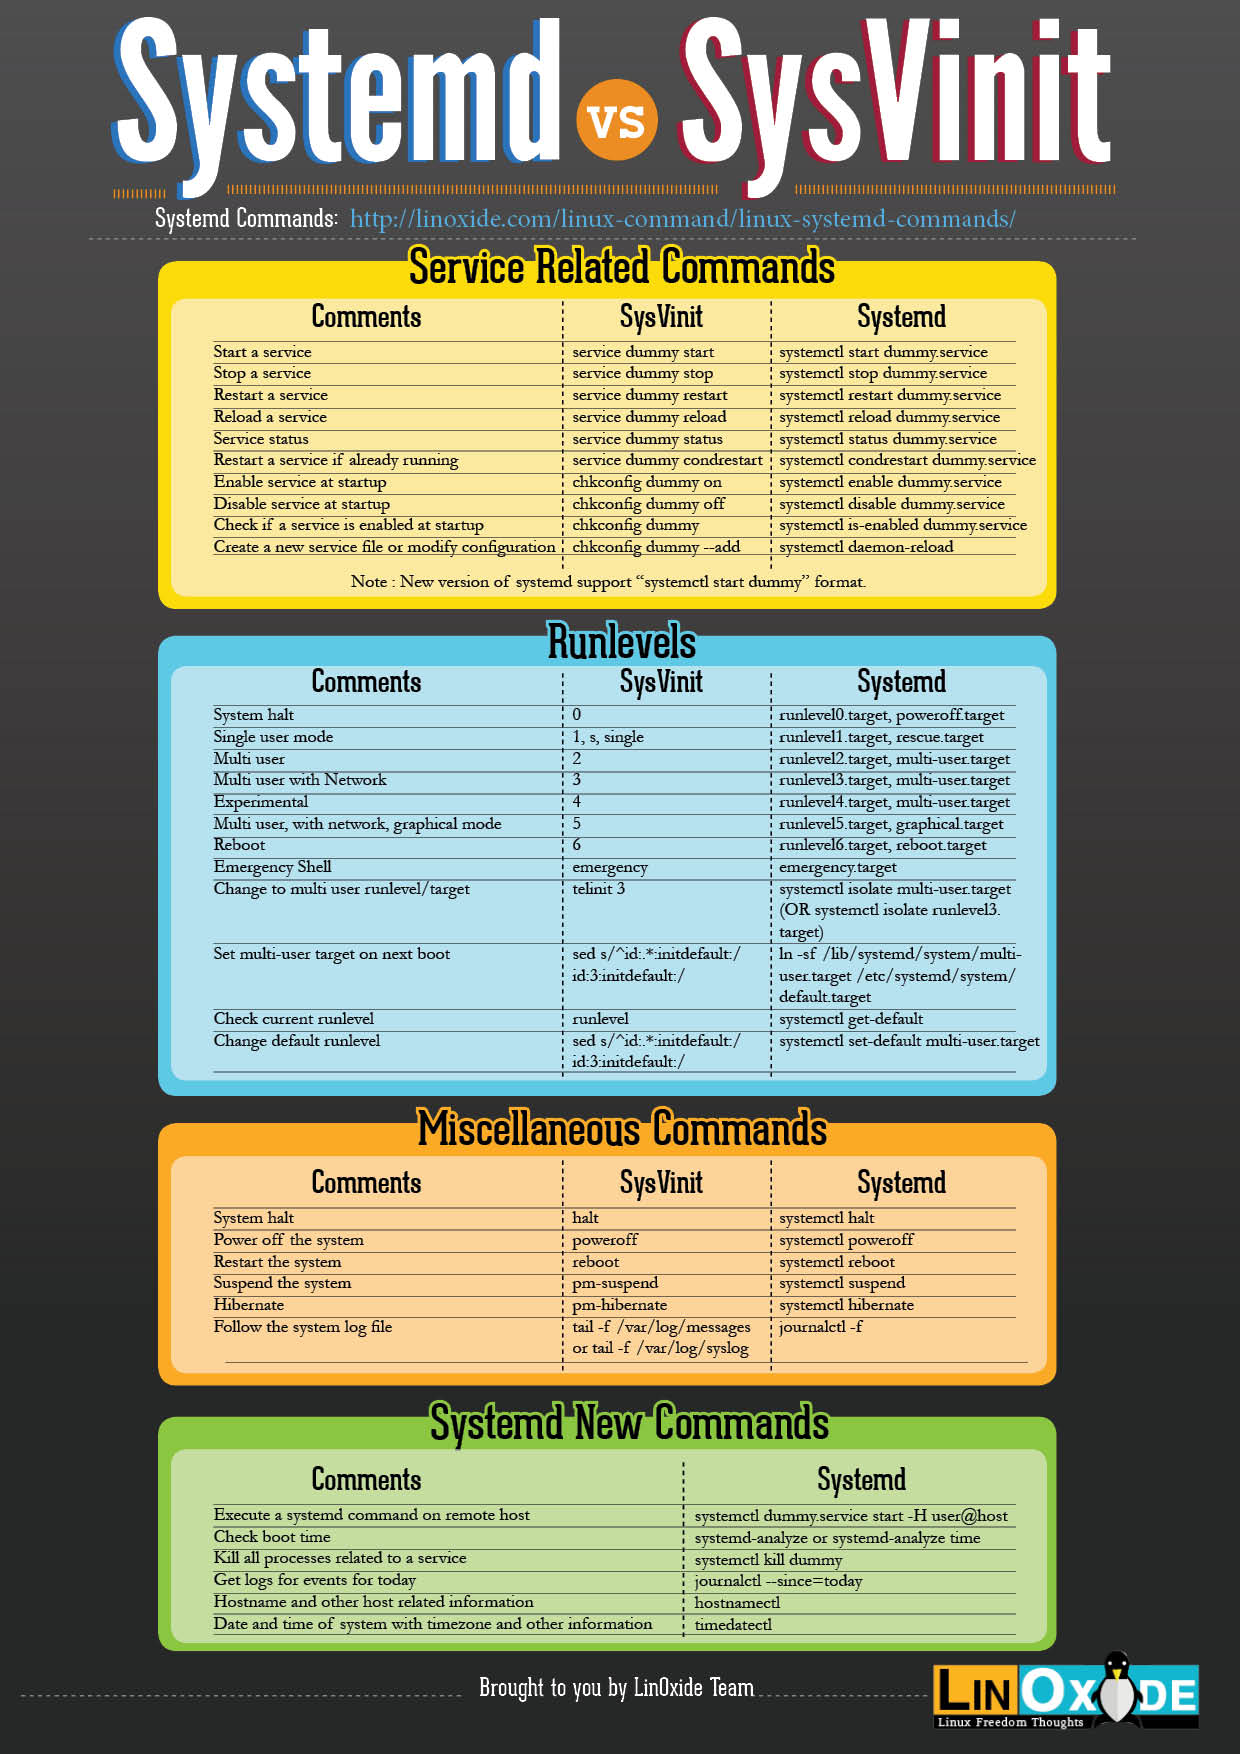
\includegraphics[scale=0.75]{./imagenes/systemd_sysVinit.png} 
\caption{Comandos de systemd vs SysVinit} \label{fig:systemd_sysVinit}
\end{figure}

%------------------------------------------------

\bibliography{citas} %archivo citas.bib que contiene las entradas 
\bibliographystyle{plain} % hay varias formas de citar

\end{document}



